\lecture{Лекция 9}{lec9}
\subtitle{Лекция 9 --- Программирование: Основные понятия}

\frame[plain]
{\titlepage}	% Титульный слайд


\begin{frame}
\frametitle{Программирование}

\begin{center}

\Huge
Основные понятия
	
\end{center}
\end{frame}

	\begin{frame}
\frametitle{Основные понятия}

\textbf{Эталонный (стандартный) язык программирования} – язык, задаваемый без относительно операционной системы и аппаратной платформы.

\textbf{Реализация языка} – диалект стандартного языка, адаптированный для данной вычислительной системы.

Минимально осмысленная для исполнителя последовательность символов называется \textbf{лексемой}.

\textbf{Конструкцией языка} называется минимальная совокупность лексем, способных вызывать действия исполнителя.

\end{frame}

	\begin{frame}
\frametitle{Основные понятия}

\textbf{Алфавит} - совокупность символов для записи конструкции языка.

\textbf{Синтаксис языка} – совокупность правил, позволяющих формально проверить корректность программы и разделить её на отдельные конструкции, а их в свою очередь на лексемы.

\textbf{Семантика} устанавливает соответствие между синтаксически правильными программами и действиями абстрактного исполнителя и позволяет определить правильность действия только исполнителя для данной программы.

\end{frame}

	\begin{frame}
\frametitle{Основные понятия}

\textbf{Императивная программа} - концепция построения языков программирования, при которой программа представляет собой однозначно интерпретируемое для исполнителя систему инструкцию, которая жестко определена программистом.

\textbf{Оператором} назовем конструкцию языка управляющими действия исполнителя или указывающие специфические требования.





\end{frame}

	\begin{frame}
\frametitle{Основные понятия}


Любая программа служит для обработки данных, которые представляются в виде специальных объектов. Для хранения данных используется \textbf{переменные и константы}.

\textbf{Переменная} представляет собой абстракцию ячеек памяти компилятора.

\textbf{Константа} это переменная жестко связанная с конкретным значением. 

В языке программирования существует специальные лексемы, которые не могут быть использованы в качестве имен переменных и называются зарезервированными словами.

\end{frame}

	\begin{frame}
\frametitle{Основные понятия}


В программировании блоком считается последовательность объявлений, определений и операторов, воспринимаемая как единое целое, составной оператор (в языке Pascal часть кода заключенная в скобки \texttt{begin end}. 

Существуют два вида блоков - составной оператор и определение функции, состоящее из составного оператора, являющегося телом функции, и предшествующего телу заголовка функции (в который входят имя функции, типы возвращаемого значения и формальных параметров). 

Блоки могут включать в себя составные операторы, но не определения функций. Внутренний блок называется вложенным, а внешний блок - объемлющим. 

\end{frame}

\begin{frame}
\frametitle{Программирование}

\begin{center}

\Huge
Переменная (variable)
	
\end{center}
\end{frame}

	\begin{frame}
\frametitle{Атрибуты переменной}



Переменную можно охарактеризовать шестеркой атрибутов:
\setlength{\columnsep}{0.4cm}
\begin{multicols}{2}
\begin{enumerate}
\item имя
\item адрес
\item значение
\item тип
\item время жизни
\item область видимости.
\end{enumerate}

\columnbreak
 
Имя переменной (константа) – это синтаксически правильная лексемой, для использования данных в программе.

\end{multicols}

\end{frame}

	\begin{frame}
\frametitle{Атрибуты переменной}



Переменную можно охарактеризовать шестеркой атрибутов:
\setlength{\columnsep}{0.4cm}
\begin{multicols}{2}
\begin{enumerate}
\item имя
\item адрес
\item значение
\item тип
\item время жизни
\item область видимости.
\end{enumerate}

\columnbreak
 
Адрес – это ячейка (ячейки) памяти, с которой связанна данная переменная. Обычно адрес это номер первой из ячеек памяти в которых хранится переменная.

\end{multicols}




\end{frame}

	\begin{frame}
\frametitle{Атрибуты переменной}



Переменную можно охарактеризовать шестеркой атрибутов:
\setlength{\columnsep}{0.4cm}
\begin{multicols}{2}
\begin{enumerate}
\item имя
\item адрес
\item значение
\item тип
\item время жизни
\item область видимости.
\end{enumerate}

\columnbreak
Значение переменной – это содержание ячеек памяти, связанной с данной переменной.
\end{multicols}

\end{frame}

	\begin{frame}
\frametitle{Атрибуты переменной}

Переменную можно охарактеризовать шестеркой атрибутов:
\setlength{\columnsep}{0.4cm}
\begin{multicols}{2}
\begin{enumerate}
\item имя
\item адрес
\item значение
\item тип
\item время жизни
\item область видимости.
\end{enumerate}

\columnbreak
 
Тип данных – это множество допустимых значений переменной вместе с набором операций над этими значениями.

\end{multicols}

\end{frame}

	\begin{frame}
\frametitle{Атрибуты переменной}

Переменную можно охарактеризовать шестеркой атрибутов:
\setlength{\columnsep}{0.4cm}
\begin{multicols}{2}
\begin{enumerate}
\item имя
\item адрес
\item значение
\item тип
\item время жизни
\item область видимости.
\end{enumerate}

\columnbreak
 \small
Время жизни переменной может быть глобальным и локальным. Переменная с глобальным временем жизни характеризуется тем, что в течение всего времени выполнения программы с ней ассоциирована ячейка памяти и значение. Переменной с локальным временем жизни выделяется новая ячейка памяти при каждом входе в блок, в котором она определена или объявлена. Время жизни функции всегда глобально. 

\end{multicols}

\end{frame}

	\begin{frame}
\frametitle{Атрибуты переменной}

Переменную можно охарактеризовать шестеркой атрибутов:
\setlength{\columnsep}{0.4cm}
\begin{multicols}{2}
\begin{enumerate}
\item имя
\item адрес
\item значение
\item тип
\item время жизни
\item область видимости.
\end{enumerate}

\columnbreak
 \small
Область видимости - это часть текста программы, в которой может быть использован данный объект. Объект считается видимым в блоке или в исходном файле, если в этом блоке или файле известны имя и тип объекта. 
\end{multicols}

\end{frame}

\begin{frame}
\frametitle{Программирование}

\begin{center}

\Huge
Тип данных
	
\end{center}
\end{frame}

	\begin{frame}
\frametitle{Тип данных}


Любой объект языка (константа, переменная и т.д.) характеризуется типом данных. Тип данных определяет:

\begin{enumerate}
	\item формат представления данных в памяти ЭВМ;
	\item множество допустимых значений;
	\item множество допустимых операций, применимых к данному типу;
	\item размер памяти выделенной для переменной (в байтах)
\end{enumerate}

\end{frame}

	\begin{frame}
\frametitle{Классификация типов данных}
Указанная классификация является в определенной мере условной.

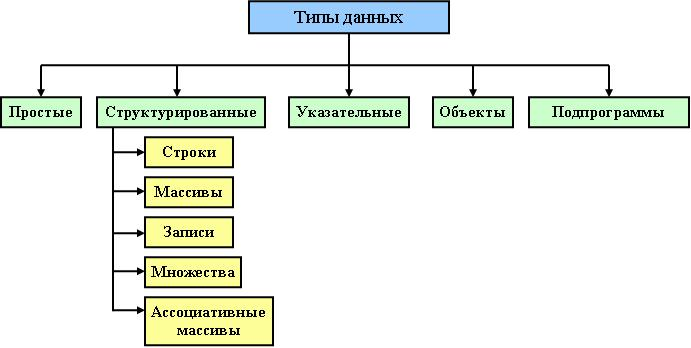
\includegraphics[height=5cm]{images/td.png}
\end{frame}

\begin{frame}
\frametitle{Программирование}

\begin{center}

\Huge
Реализация языков программирования
	
\end{center}
\end{frame}

	\begin{frame}
\frametitle{Реализация языков программирования}


Любой ЯВУ существует в виде так называемого обобщенного языка, ориентированного на абстрактного исполнителя и определяемого в формальной спецификации. 

Для конкретной аппаратной платформы создается реализация языка, которая поддерживается системой программирования.

\end{frame}

	\begin{frame}
\frametitle{Основные компоненты системы программирования}


\textbf{Редактор} – служит для ввода, редактирования программы.

\textbf{Транслятор} – комплекс программ, преобразующий текст программы к виду, в котором она может выполняться, и указания ошибок в случаи неудач. Синонимом транслятора служит компилятор , который преобразует текст программы в машинные коды. Результат работы компилятора – загрузочный модуль.

Альтернативой компилятора является \textbf{интерпретатор}, который выполняет программу по мере её ввода.

\end{frame}

	\begin{frame}
\frametitle{Основные компоненты системы программирования}


\textbf{Библиотеки подпрограмм}, которые внедряются в загрузочный модуль на этапе трансляции, и служат для выполнения стандартизированных операций.

\textbf{Отладчик} – программа, позволяющая отследить ход вычисления на данном языке программирования.

\textbf{Средства поддержки разработки программ} – комплекс инструментальных средств, которые применяются в процессе проектировании, составлении и отладки программ..

\end{frame}